\author{Patrick Bucher}
\title{DeepXRay}
\subtitle{Bachelorarbeit, Frühlingssemester 2020, HSLU ‒ Informatik}
\date{\today}
\maketitle
\thispagestyle{empty}

\begin{center}
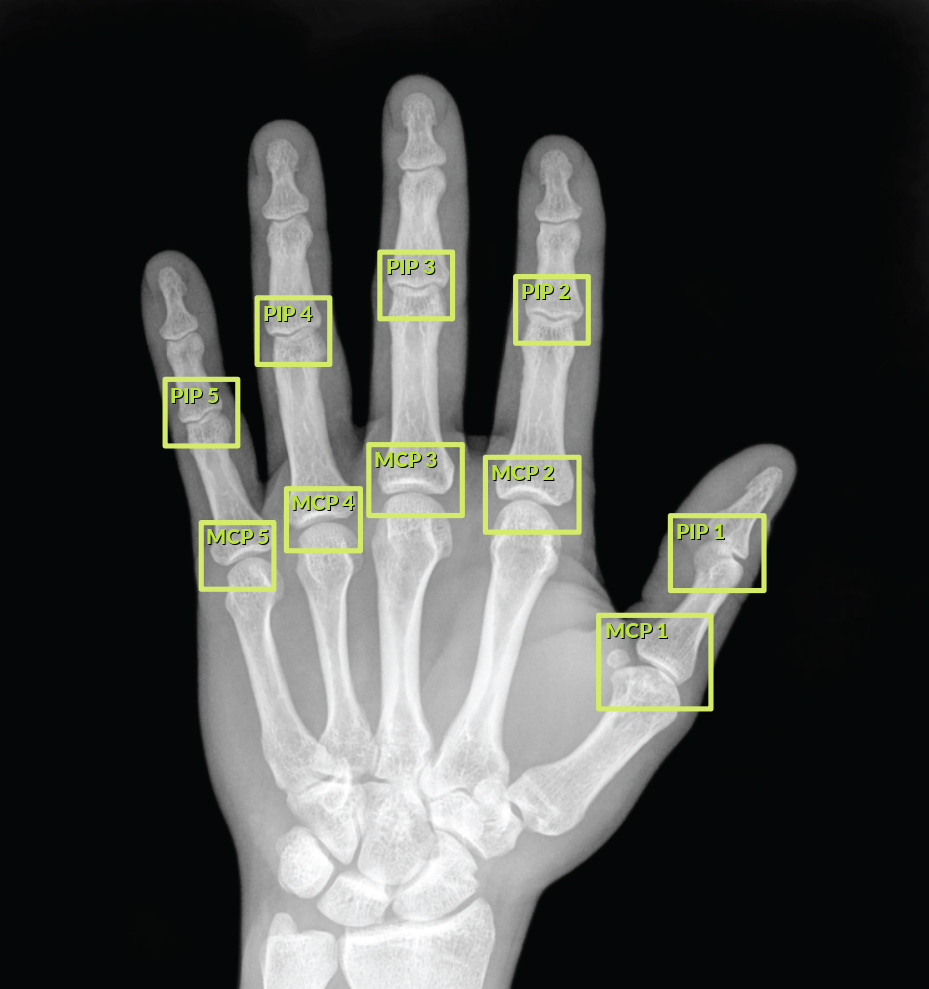
\includegraphics[width=0.75\linewidth]{pics/xray-left-hand-annotated.png}
\end{center}

\vfill

\begin{multicols}{3}
    \center

    \noindent
    \textsc{\textbf{Auftraggeber}} \\ Dr. Tobias Reinhard \\ Seantis GmbH

    \noindent
    \textsc{\textbf{Betreuer}} \\ Daniel Pfäffli \\ HSLU ‒ Informatik

    \noindent
    \textsc{\textbf{Experte}} \\ Jeremy Callner \\ APG|SGA
\end{multicols}

\newpage
\thispagestyle{empty}

{
\setlength{\parindent}{0cm}
\setlength{\parskip}{13pt}

\textbf{Bachelorarbeit an der Hochschule Luzern ‒ Informatik}

\textbf{Titel:} DeepXRay

\textbf{Student:} Patrick Bucher

\textbf{Studiengang:} BSc Informatik

\textbf{Jahr:} 2020

\textbf{Betreuungsperson:} Daniel Pfäffli, HSLU ‒ Informatik

\textbf{Experte:} Jeremy Callner, APG|SGA

\textbf{Auftraggeber:} Tobias Reinhard, Seantis GmbH

\textbf{Codierung/Klassifizierung der Arbeit:}

$\boxtimes$ A: Einsicht \tabto{3.5cm}    (Normalfall) \\
$\square$ B: Rücksprache \tabto{3.5cm} (Dauer: \underline{\hspace*{0.5cm}} Jahr/Jahre) \\
$\square$ C: Sperre \tabto{3.5cm}      (Dauer: \underline{\hspace*{0.5cm}} Jahr/Jahre)

\paragraph{\textbf{Eidesstattliche Erklärung}}

Ich erkläre hiermit, dass ich die vorliegende Arbeit selbständig und ohne unerlaubte fremde Hilfe angefertigt habe, alle verwendeten Quellen, Literatur und andere Hilfsmittel angegeben habe, wörtlich oder inhaltlich entnommene Stellen als solche kenntlich gemacht habe, das Vertraulichkeitsinteresse des Auftraggebers wahre und die Urheberrechtsbestimmungen der Fachhochschule Zentralschweiz (siehe Merkblatt «Studentische Arbeiten» auf MyCampus) respektieren werde.

\vspace{13pt}

Ort/Datum, Unterschrift \hspace{0.25cm} \underline{\hspace*{9cm}} 

\newpage
\thispagestyle{empty}

\textbf{Abgabe der Arbeit auf der Portfolio-Datenbank:}

Bestätigungsvisum Student

Ich bestätige, dass ich die Bachelorarbeit korrekt gemäss Merkblatt auf der Portfolio-Datenbank abgelegt habe. Die Verantwortlichkeit sowie die Berechtigungen habe ich abgegeben, so dass ich keine Änderungen mehr vornehmen kann oder weitere Dateien hochladen kann.

Ort/Datum, Unterschrift \hspace{0.25cm} \underline{\hspace*{9cm}} 

\textbf{Verdankung}

Ich bedanke mich bei meinem Arbeitgeber Seantis GmbH, insbesondere beim Auftraggeber Dr. Tobias Reinhard dafür, dass ich die Möglichkeit erhalten habe, eine interessante und herausfordernde Arbeit im Umfeld der Firma erstellen zu dürfen, und für die Hilfestellungen im Verlauf der Arbeit. Bei der SCQM bedanke ich mich für die zur Verfügung gestellten Röntgenbilder, die mir als Evaluationsdaten dienten. Bei Janick Rohrbach und Dr. Tobias Reinhard bedanke ich mich für ihre Vorarbeit im Bereich Machine Learning, ohne die das vorliegende Projekt nicht möglich gewesen wäre.

{\textbf{Ausschliesslich bei Abgabe in gedruckter Form:\\
Eingangsvisum durch das Sekretariat auszufüllen}}

Rotkreuz, den \underline{\hspace*{4cm}} \hspace*{1cm} Visum: \underline{\hspace*{4cm}}

\vspace*{\fill}

{
\small
\setlength{\parskip}{11pt}
{\textbf{Hinweis}}: Die Bachelorarbeit wurde von keinem Dozierenden nachbearbeitet. Veröffentlichungen (auch auszugsweise) sind ohne das Einverständnis der Studiengangleitung der Hochschule Luzern ‒ Informatik nicht erlaubt.

\textbf{Copyright} \textcopyright\ 2020 Hochschule Luzern ‒ Informatik

Alle Rechte vorbehalten. Kein Teil dieser Arbeit darf ohne die schriftliche Genehmigung der Studiengangleitung der Hochschule Luzern ‒ Informatik in irgendeiner Form reproduziert oder in eine von Maschinen verwendete Sprache übertragen werden.
}

} % setlength parindent
